

\tikzset{every picture/.style={line width=0.75pt}} %set default line width to 0.75pt        
\resizebox{\textwidth}{!}{%
\begin{tikzpicture}[x=0.75pt,y=0.75pt,yscale=-1,xscale=1,font=\sffamily]
%uncomment if require: \path (0,435); %set diagram left start at 0, and has height of 435

%Image [id:dp612682770859811] 
\draw (251.86,178.3) node  {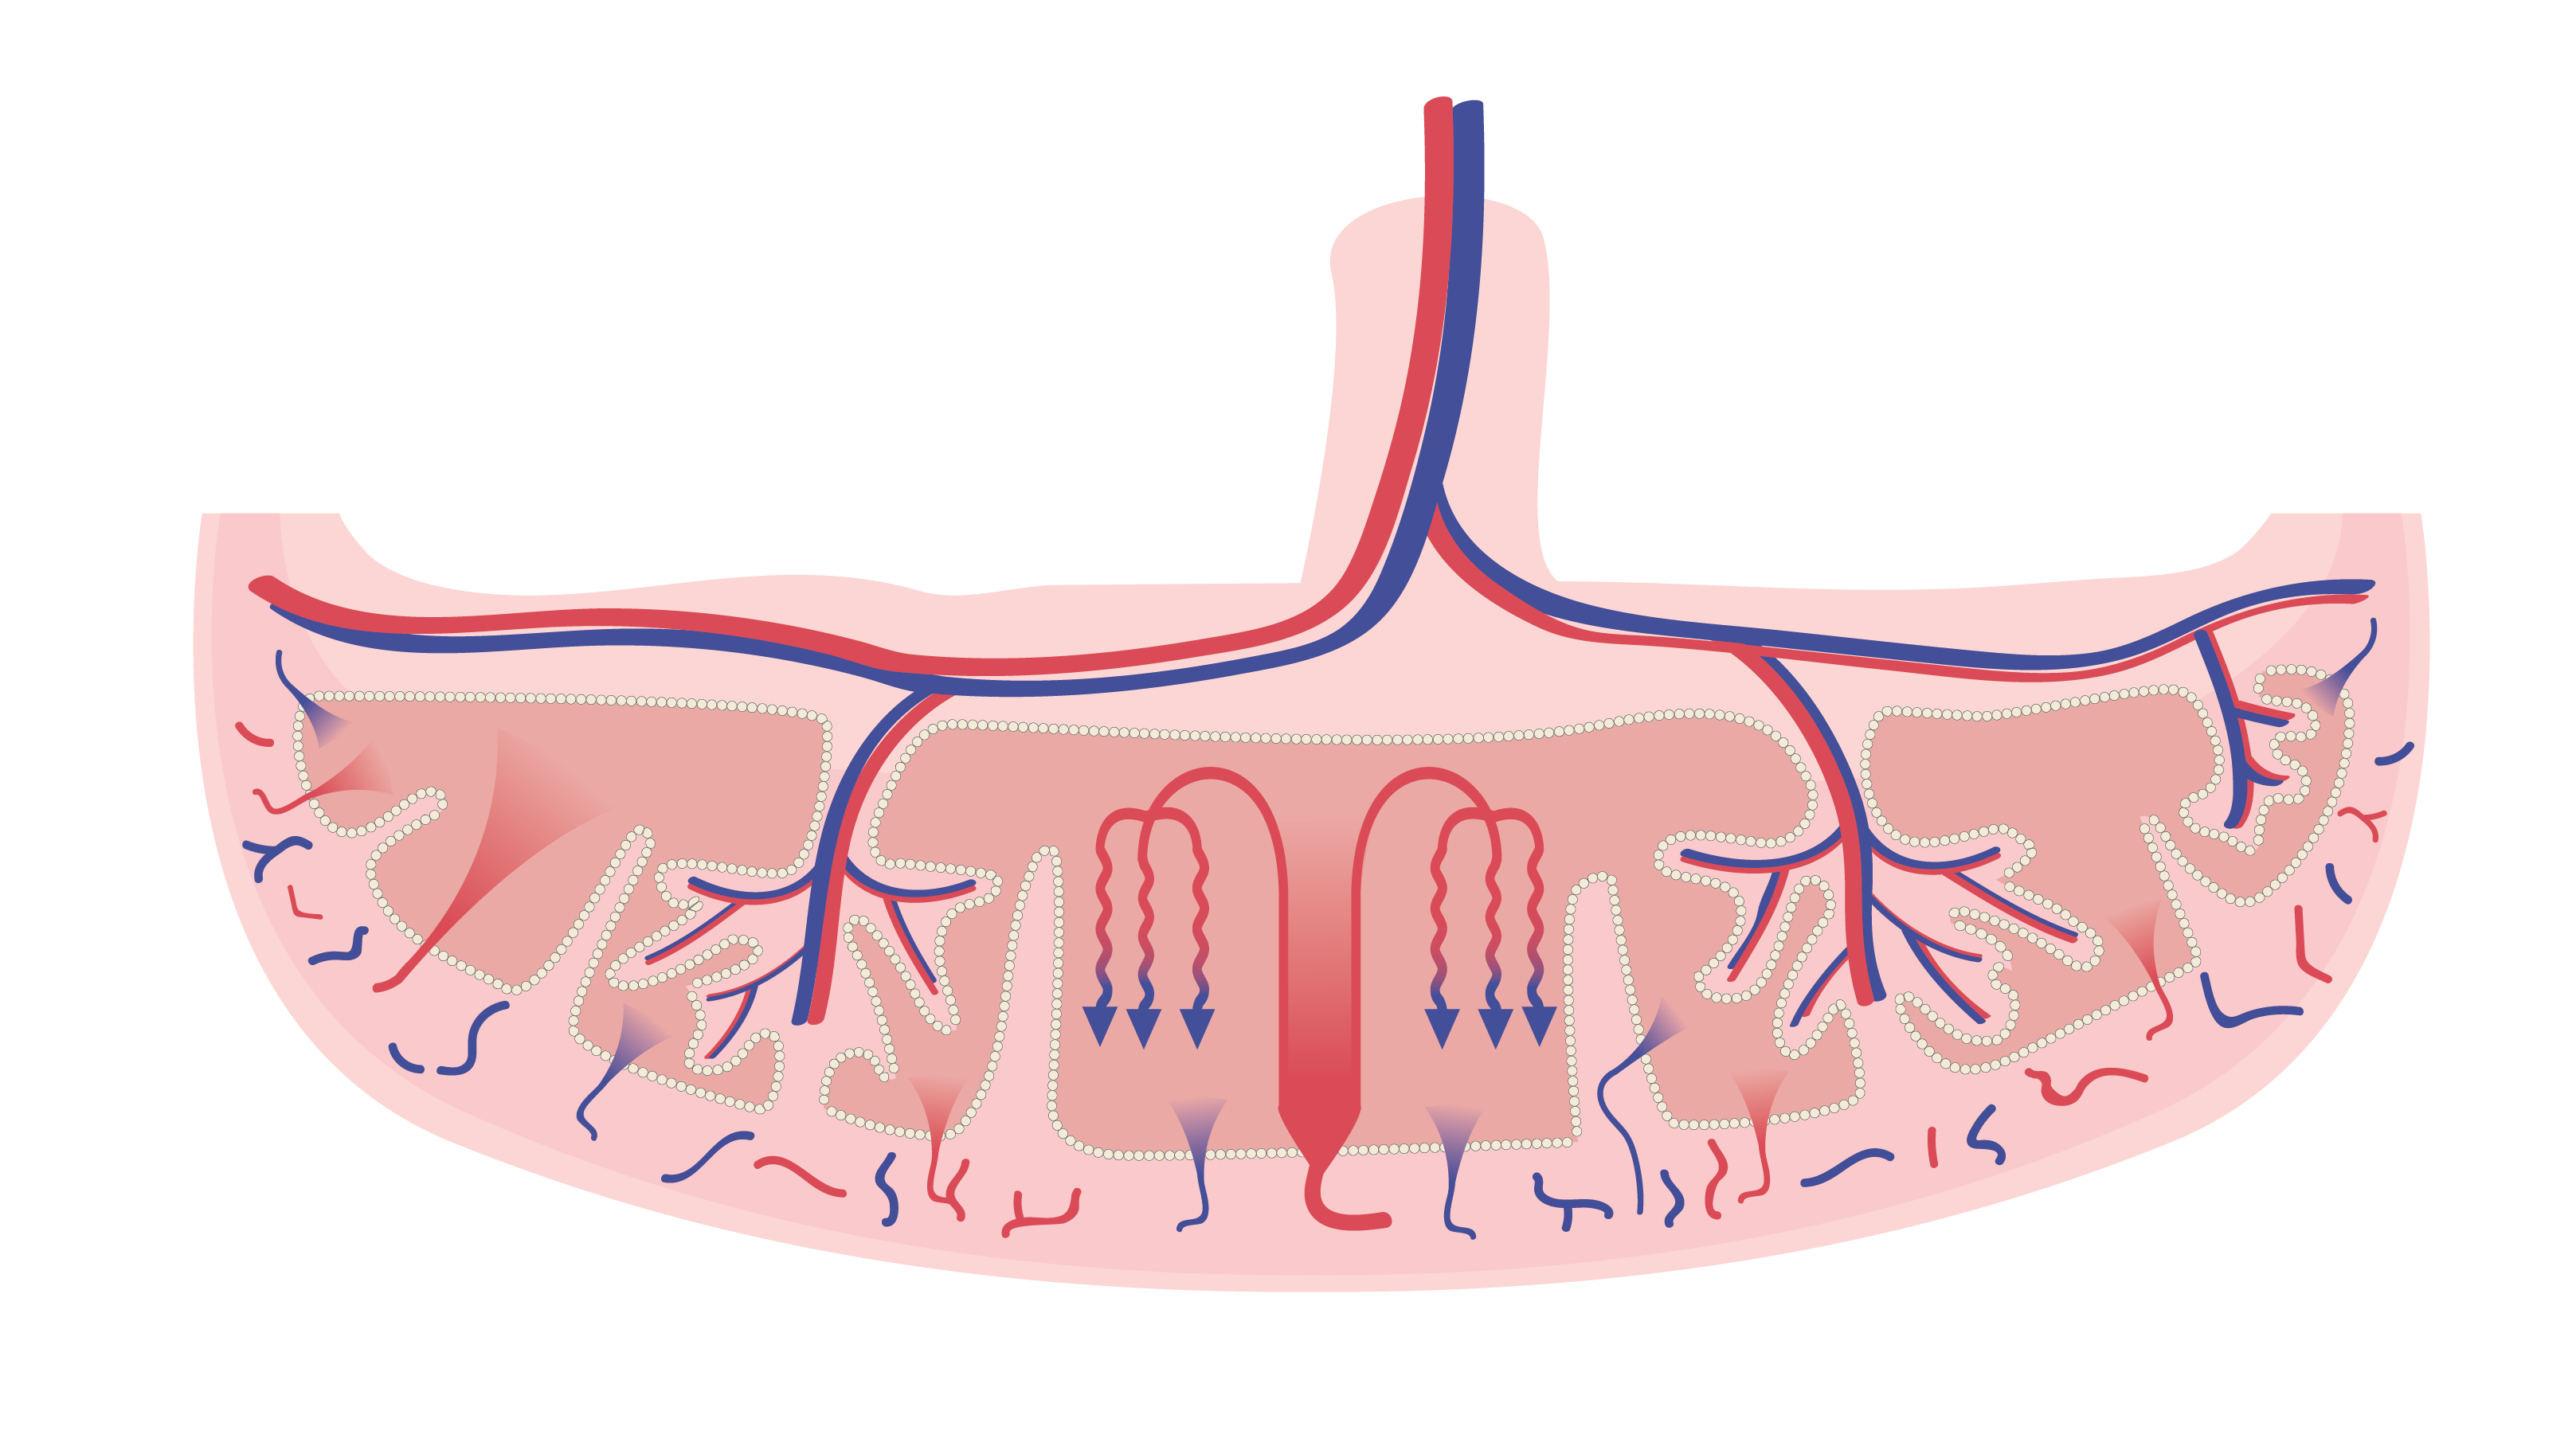
\includegraphics[width=399.29pt,height=225.45pt]{diagrams/placenta-geometry-diagrams/placenta-cartoon-2024.png}};
%Straight Lines [id:da3701239304155397] 
\draw [color={rgb, 255:red, 71; green, 153; blue, 84 }  ,draw opacity=1 ][line width=1.5]    (438,136.13) -- (69.29,136.13) ;
\draw [shift={(65.29,136.13)}, rotate = 360] [fill={rgb, 255:red, 71; green, 153; blue, 84 }  ,fill opacity=1 ][line width=0.08]  [draw opacity=0] (11.61,-5.58) -- (0,0) -- (11.61,5.58) -- cycle    ;
\draw [shift={(442,136.13)}, rotate = 180] [fill={rgb, 255:red, 71; green, 153; blue, 84 }  ,fill opacity=1 ][line width=0.08]  [draw opacity=0] (11.61,-5.58) -- (0,0) -- (11.61,5.58) -- cycle    ;
%Shape: Arc [id:dp7839630490555429] 
\draw  [draw opacity=0][line width=1.5]  (487.26,230.95) .. controls (487.54,232.37) and (487.68,233.81) .. (487.68,235.27) .. controls (487.68,274.09) and (385.83,305.56) .. (260.18,305.56) .. controls (134.53,305.56) and (32.67,274.09) .. (32.67,235.27) -- (260.18,235.27) -- cycle ; \draw [color={rgb, 255:red, 71; green, 153; blue, 84 }  ,draw opacity=1 ][line width=1.5]    (487.68,234.94) .. controls (487.68,235.05) and (487.68,235.16) .. (487.68,235.27) .. controls (487.68,274.09) and (385.83,305.56) .. (260.18,305.56) .. controls (138.3,305.56) and (38.81,275.95) .. (32.95,238.74) ; \draw [shift={(32.67,235.27)}, rotate = 84.01] [fill={rgb, 255:red, 71; green, 153; blue, 84 }  ,fill opacity=1 ][line width=0.08]  [draw opacity=0] (11.61,-5.58) -- (0,0) -- (11.61,5.58) -- cycle    ; \draw [shift={(487.26,230.95)}, rotate = 94.26] [fill={rgb, 255:red, 71; green, 153; blue, 84 }  ,fill opacity=1 ][line width=0.08]  [draw opacity=0] (11.61,-5.58) -- (0,0) -- (11.61,5.58) -- cycle    ;
%Straight Lines [id:da8876380274555917] 
\draw [line width=1.5]    (181.85,82.47) -- (251.5,82.47) ;
\draw [shift={(255.5,82.47)}, rotate = 180] [fill={rgb, 255:red, 0; green, 0; blue, 0 }  ][line width=0.08]  [draw opacity=0] (11.61,-5.58) -- (0,0) -- (11.61,5.58) -- cycle    ;
%Straight Lines [id:da3261920772723992] 
\draw [line width=1.5]    (386,97.81) -- (334.04,185.37) ;
\draw [shift={(332,188.81)}, rotate = 300.69] [fill={rgb, 255:red, 0; green, 0; blue, 0 }  ][line width=0.08]  [draw opacity=0] (11.61,-5.58) -- (0,0) -- (11.61,5.58) -- cycle    ;
%Straight Lines [id:da23004860167795904] 
\draw [color={rgb, 255:red, 124; green, 71; blue, 153 }  ,draw opacity=1 ][line width=1.5]    (421,310.31) -- (376.68,240.74) ;
\draw [shift={(374.53,237.37)}, rotate = 57.5] [fill={rgb, 255:red, 124; green, 71; blue, 153 }  ,fill opacity=1 ][line width=0.08]  [draw opacity=0] (11.61,-5.58) -- (0,0) -- (11.61,5.58) -- cycle    ;
%Straight Lines [id:da26234807553589] 
\draw [color={rgb, 255:red, 218; green, 75; blue, 87 }  ,draw opacity=1 ][line width=1.5]    (260.68,314.42) -- (260.68,290.32) ;
\draw [shift={(260.68,286.32)}, rotate = 90] [fill={rgb, 255:red, 218; green, 75; blue, 87 }  ,fill opacity=1 ][line width=0.08]  [draw opacity=0] (11.61,-5.58) -- (0,0) -- (11.61,5.58) -- cycle    ;
%Straight Lines [id:da659245707576972] 
\draw [color={rgb, 255:red, 71; green, 85; blue, 153 }  ,draw opacity=1 ][line width=1.5]    (353.5,344.31) -- (326.23,255.23) ;
\draw [shift={(325.05,251.4)}, rotate = 72.98] [fill={rgb, 255:red, 71; green, 85; blue, 153 }  ,fill opacity=1 ][line width=0.08]  [draw opacity=0] (11.61,-5.58) -- (0,0) -- (11.61,5.58) -- cycle    ;
%Straight Lines [id:da0549441454891868] 
\draw [color={rgb, 255:red, 248; green, 140; blue, 147 }  ,draw opacity=1 ][line width=1.5]    (177,344.81) -- (195.28,263.52) ;
\draw [shift={(196.15,259.62)}, rotate = 102.67] [fill={rgb, 255:red, 248; green, 140; blue, 147 }  ,fill opacity=1 ][line width=0.08]  [draw opacity=0] (11.61,-5.58) -- (0,0) -- (11.61,5.58) -- cycle    ;
%Straight Lines [id:da750105190473205] 
\draw [color={rgb, 255:red, 71; green, 85; blue, 153 }  ,draw opacity=1 ][line width=1.5]    (454,121.81) -- (466.77,161.26) ;
\draw [shift={(468,165.06)}, rotate = 252.06] [fill={rgb, 255:red, 71; green, 85; blue, 153 }  ,fill opacity=1 ][line width=0.08]  [draw opacity=0] (11.61,-5.58) -- (0,0) -- (11.61,5.58) -- cycle    ;
%Image [id:dp6947304444659705] 
\draw (285.83,93.75) node  {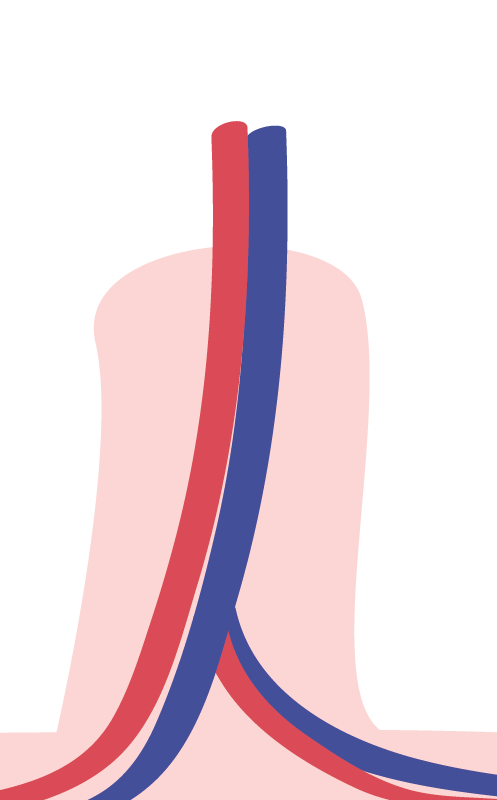
\includegraphics[width=61.5pt,height=98.99pt]{diagrams/placenta-geometry-diagrams/placenta-cartoon-2024_uc.png}};
%Straight Lines [id:da1217993864688609] 
\draw [color={rgb, 255:red, 71; green, 85; blue, 153 }  ,draw opacity=1 ][line width=1.5]    (113.55,313.31) -- (113.55,262.4) ;
\draw [shift={(113.55,258.4)}, rotate = 90] [fill={rgb, 255:red, 71; green, 85; blue, 153 }  ,fill opacity=1 ][line width=0.08]  [draw opacity=0] (11.61,-5.58) -- (0,0) -- (11.61,5.58) -- cycle    ;

% Text Node
\draw (180.89,82) node [anchor=east] [inner sep=0.75pt]   [align=left] {Umbilical cord};
% Text Node
\draw (167.71,128.99) node [anchor=south] [inner sep=0.75pt]  [color={rgb, 255:red, 71; green, 153; blue, 84 }  ,opacity=1 ] [align=left] {Chorionic plate};
% Text Node
\draw (386,94.81) node [anchor=south] [inner sep=0.75pt]   [align=left] {Intervillous space (IVS)};
% Text Node
\draw (421,313.31) node [anchor=north] [inner sep=0.75pt]  [color={rgb, 255:red, 124; green, 71; blue, 153 }  ,opacity=1 ] [align=left] {Villous tree};
% Text Node
\draw (260.68,316.83) node [anchor=north] [inner sep=0.75pt]  [color={rgb, 255:red, 218; green, 75; blue, 87 }  ,opacity=1 ] [align=left] {Spiral artery};
% Text Node
\draw (64.67,279.61) node [anchor=north] [inner sep=0.75pt]  [color={rgb, 255:red, 71; green, 153; blue, 84 }  ,opacity=1 ,rotate=-24.27] [align=left] {Basal plate};
% Text Node
\draw (177,347.81) node [anchor=north] [inner sep=0.75pt]  [color={rgb, 255:red, 248; green, 140; blue, 147 }  ,opacity=1 ] [align=left] {Septal wall};
% Text Node
\draw (454,118.81) node [anchor=south] [inner sep=0.75pt]  [color={rgb, 255:red, 71; green, 85; blue, 153 }  ,opacity=1 ] [align=left] {Marginal sinus vein};
% Text Node
\draw (353.5,347.31) node [anchor=north] [inner sep=0.75pt]  [color={rgb, 255:red, 71; green, 85; blue, 153 }  ,opacity=1 ] [align=left] {Septal wall vein};
% Text Node
\draw (113.55,316.31) node [anchor=north] [inner sep=0.75pt]  [color={rgb, 255:red, 71; green, 85; blue, 153 }  ,opacity=1 ] [align=left] {Basal plate vein};



\end{tikzpicture}
}